\documentclass[aps,prd,onecolumn,superscriptaddress,nofootinbib]{revtex4-2}

% — Packages —
\usepackage[utf8]{inputenc}
\usepackage[T1]{fontenc}
\usepackage{lmodern}
\usepackage{amsmath,amssymb,bm,mathtools,amsthm}
\usepackage{graphicx}
\usepackage{adjustbox}
\usepackage{xcolor}
\usepackage{microtype}
\usepackage[unicode, pdfencoding=auto, psdextra]{hyperref}
\usepackage{enumitem}
\usepackage{tikz}
\usepackage{booktabs}
\usepackage{siunitx}
\sisetup{detect-all}
\usetikzlibrary{arrows.meta,positioning,fit,calc,shapes.geometric,shapes.multipart,backgrounds}

% — Colors for flowchart —
\definecolor{flowBlue}{HTML}{1F77B4}
\definecolor{flowPurple}{HTML}{9467BD}
\definecolor{flowGreen}{HTML}{2CA02C}
\definecolor{flowOrange}{HTML}{FF7F0E}
\definecolor{flowRed}{HTML}{D62728}
\definecolor{flowGray}{HTML}{7F7F7F}

% — Hyperref —
\hypersetup{
  colorlinks=true,
  linkcolor=blue,
  citecolor=blue,
  urlcolor=blue
}

% — PDF string sanitization —
\pdfstringdefDisableCommands{%
  \def\OmL{OmegaLambda}%
  \def\Omm{Omega m0}%
  \def\cgeo{cgeo}%
  \def\alphaM{alphaM}%
  \def\eps{epsilon}%
  \def\boxed#1{#1}%
  \def\mu{mu}%
  \def\alpha{alpha}%
  \def\alpha_M{alphaM}%
  \def\Omega_\Lambda{OmegaLambda}%
}

% — Math tweaks —
\allowdisplaybreaks

% — Macros —
\providecommand{\mpl}{M_{\rm P}}
\providecommand{\OmL}{\Omega_\Lambda}
\providecommand{\Omm}{\Omega_{m0}}
\providecommand{\cgeo}{c_{\rm geo}}
\providecommand{\alphaM}{\alpha_M}
\providecommand{\eps}{\varepsilon}
\providecommand{\be}{\begin{equation}}
\providecommand{\ee}{\end{equation}}
\providecommand{\bse}{\begin{subequations}}
\providecommand{\ese}{\end{subequations}}

% — Theorem-like environments —
\newtheorem{definition}{Definition}
\newtheorem{hypothesis}{Hypothesis}
\newtheorem{lemma}{Lemma}
\newtheorem{proposition}{Proposition}
\newtheorem{theorem}{Theorem}
\newtheorem{corollary}{Corollary}

\begin{document}

\title{Modular Response in Free Quantum Fields:\\
A KMS/FDT Theorem and Conditional Extensions}

\author{[Authors]}
\affiliation{[Institutions]}
\date{}

\begin{abstract}
\textbf{Part I (Theoremic core, free/Gaussian Hadamard QFT).} We prove that, for small causal diamonds (CHM) in locally Hadamard states and within a safe window \(\epsilon_{\rm UV}\ll\ell\ll \min\{L_{\rm curv},\lambda_{\rm mfp},m_i^{-1}\}\), the MI/moment-kill projector isolates a finite \(\ell^4\) modular response with coefficient equal to its flat-space value; the projected KMS/FDT susceptibility is positive; and coarse-graining over the wedge family produces the universal weak-field prefactor \(5/12=(4/3)\times(5/16)\). The fractional KMS defect between CHM diamonds and half-spaces scales as \(\mathcal O((\ell/L_{\rm curv})^2)+\mathcal O((\ell H)^2)\). The QFT sensitivity is \(\beta=2\pi C_T I_{00}=0.02086\pm 0.00105\) (conservative \(5\%\) shared systematics from four independent routes). A scheme-invariant background relation \emph{suggests} \(\OmL=\beta\, f\,\cgeo\) \emph{conditional} on our coarse-graining and analyticity assumptions.

\smallskip
\textbf{Part II (Conditional extensions).} We separate \emph{definition} (flat-space \(\eps\) from modular response) from \emph{mapping}. Rather than impose the standard EFT-of-DE \(\alpha\)-basis, we adopt a quasi-static closure that keeps operational distances GR-like (no additional lensing coupling \(\Sigma\simeq 1\)) while modifying growth via \(\mu(\eps)=1/(1+\tfrac{5}{12}\eps)\). KMS/FDT positivity motivates an entropy-driven law \(d\eps/d\ln a\ge 0\) with a \emph{conditional} background budget \(\int \eps\,d\ln a=\OmL\). We introduce a covariant environment envelope \(F_g(\chi_g)=[1+(\chi_g/\chi_\star)^q]^{-1}\) with \(\chi_g\equiv \ell^2\sqrt{C_{abcd}C^{abcd}}\), calibrated by Solar-System bounds. Cosmological illustrations (\(S_8\) band and \(H_0\) bounds) are \textbf{toy/illustrative} and propagate the \(\pm5\%\) \(\beta\) uncertainty; \emph{observed lensing amplitudes still reflect the altered growth}.

\smallskip
\emph{What is new.} (i) Completed proofs in the Gaussian/Hadamard sector; (ii) a \textbf{conditional, coarse-grained} KMS\(\to\)FRW averaging statement with explicit error budget; (iii) \textbf{Assumptions C and D stated with rationale} (relative entropy \(\leftrightarrow\) canonical energy in the projected diamond; uniqueness of \(M^2\) at working order), with proofs deferred; (iv) semi-analytic quantification of the safe-window volume fraction \(f_V(\ell_{\min})\); (v) a symmetry-constrained \(F_g\) envelope; (vi) uncertainty propagation of \(\beta\) into \(S_8\) and \(H_0\) \emph{illustrations}; (vii) a preliminary entropic derivation (App.~\ref{app:entropic-proof}) linking KMS positivity to FRW evolution.
\end{abstract}

\maketitle

% ============================================================
\section*{Reader’s map: Part I (Theorem) vs.\ Part II (Conditional)}
\noindent \textbf{Part I (Secs.~\ref{sec:scope}–\ref{sec:five-twelve}, Apps.~\ref{app:MI}–\ref{app:chm-kms-estimate}):} proven results for free/Gaussian Hadamard fields at working order.\\
\textbf{Part II (Secs.~\ref{sec:def-vs-map}–\ref{sec:data}, Apps.~\ref{app:fv}–\ref{app:microlocal}, \ref{app:entropic-proof}):} conditional extensions, Assumptions C \& D (stated), safe-window fraction, KMS\(\to\)FRW link, symmetry envelope, entropic sketch, and toy/illustrative numerics with propagated uncertainties.

% ===============================
\section{Scope, Working Order, and Safe-Window Quantification (Part I)}
\label{sec:scope}

\paragraph{Working order and state class.} We work to \(\mathcal O(\ell^4)\) in the MI/moment-kill projector channel, treating curvature/contact terms as \(\mathcal O(\ell^6)\). States are locally Hadamard.

\paragraph{KMS applicability (CHM diamonds).} Exact BW KMS holds for half-spaces; CHM diamonds inherit it with fractional defect \(\mathcal O((\ell/L_{\rm curv})^2)+\mathcal O((\ell H)^2)\) (App.~\ref{app:chm-kms-estimate}).

\paragraph{Safe-window volume fraction.} Define a conservative admissible scale
\be
\label{eq:lmax}
\ell_{\max}(x)\equiv \zeta\;\min\Big\{L_{\rm curv}(x),\ \lambda_{\rm mfp}(x),\ m_i^{-1}(x)\Big\},\qquad \zeta=0.1.
\ee
Using Press--Schechter/Sheth--Tormen mass functions and NFW curvature proxies \(L_{\rm curv}^{-2}\sim (R_{abcd}R^{abcd})^{1/2}\) with substructure excision parameter \(\xi\), we estimate the comoving volume fraction \(f_V(\ell_{\min})=\mathrm{Vol}\{x:\,\ell_{\max}(x)>\ell_{\min}\}/\mathrm{Vol}_{\rm tot}\). A semi-analytic survey (App.~\ref{app:fv}) shows voids dominate \(f_V\), while dense cores lack a window; representative values at \(z\!\sim\!0\) for \(\ell_{\min}\in[1,100]\) pc are \(f_V\sim 0.6{-}0.95\) for \(\xi\in[0.2,0.5]\). This enters only as a domain-of-validity indicator.

\paragraph{Angle invariance as a null test.} The continuous-angle product \(\mathcal C_\Omega=f(\theta)\,\cgeo(\theta)\) is analytic and \(\theta\)-independent; residuals are shown as a null check, not a precision claim.

% ===============================
\section{A2–KMS Theorem (Gaussian/Hadamard Sector)}
\label{sec:theorem}

\begin{theorem}[Projected modular response and positivity]\label{thm:proj-modresp}
Let \(\mathcal Q\) be a free (Gaussian) QFT on a globally hyperbolic spacetime and \(\rho\) a locally Hadamard state. For a causal diamond of radius \(\ell\) with \(\ell\ll L_{\rm curv}\) and the MI/moment-kill projector that cancels \(r^0\) and \(r^2\) moments, the MI-subtracted modular response obeys
\be
\delta\!\langle K_{\rm sub}\rangle=(2\pi C_T I_{00})\,\ell^4\,\delta\eps+\mathcal O(\ell^6),
\ee
with coefficient equal to the flat-space value. The retarded susceptibility \(\chi_{QK}\) in the projected channel is positive (FDT), and wedge averaging yields the universal weak-field prefactor \(5/12\). The fractional deviation from BW KMS is \(\mathcal O((\ell/L_{\rm curv})^2)+\mathcal O((\ell H)^2)\).
\end{theorem}

\begin{corollary}[Conditional background statement]\label{cor:background-cond}
Under the coarse-graining and analyticity assumptions of Sec.~\ref{sec:kms-frw}, the FRW zero mode \emph{suggests} the scheme-invariant relation
\(\OmL=\beta\,f\,\cgeo\) with \(\beta=2\pi C_T I_{00}\). We treat this as a conditional statement rather than a theorem.
\end{corollary}

% ===============================
\section{QFT Input: \texorpdfstring{$\beta=2\pi C_T I_{00}$}{beta} and Error Budget}
\label{sec:beta}
We evaluate \(\beta\) via four independent routes: (a) real-space CHM; (b) spectral/Bessel; (c) Euclidean time-slicing; (d) replica finite-difference. The spread is \(\lesssim 1\%\). We adopt a conservative
\be
\beta=0.02086\pm 0.00105 \quad (5\%~\text{shared systematics}).
\ee
Angle invariance is used as a null residual test.

\noindent Here \(C_T\) denotes the flat-space stress-tensor two-point normalization, e.g.
\(\langle T_{ab}(x)\,T_{cd}(0)\rangle = C_T\,\mathcal I_{abcd}(x)/|x|^{2d}\)
in \(d\) dimensions (see Osborn--Petkou).

\noindent\emph{Benchmark (convention).} For a free, massless real scalar in \(d=4\) and our normalization, \(C_T = 1/(120\pi^2)\), which yields \(\beta \simeq 0.02086\) via Eq.~\eqref{eq:eps-def}.

% ===============================
\section{Weak-Field Prefactor \texorpdfstring{$5/12$}{5/12}}
\label{sec:five-twelve}
The isotropic BW channel gives \(\langle T_{kk}\rangle=(1+w)\rho\) with UV \(w=1/3\Rightarrow 4/3\). Averaging over CHM segments yields \(5/16\), so \(5/12=(4/3)\times(5/16)\). Details in App.~\ref{app:five-twelve}.

% ============================================================
\section{Definition vs.\ Mapping (Part II; Conditional)}
\label{sec:def-vs-map}

\paragraph{Definition (flat-space QFT).}
\be
\label{eq:eps-def}
\delta\!\langle K_{\rm sub}(\ell)\rangle=\underbrace{(2\pi C_T I_{00})}_{\beta}\,\ell^4\,\delta\eps(x)+\mathcal O(\ell^6).
\ee

\paragraph{Mapping (constitutive; beyond the \texorpdfstring{$\alpha$}{alpha}-basis).}
We \emph{do not} impose the linear EFT-of-DE $\alpha$-parameter mapping at working order. Instead, we adopt a quasi-static closure that keeps operational distances GR-like while modifying growth:
\bse
\label{eq:qs-closure}
\be
\nabla^2\Phi \;=\; 4\pi G a^2 \rho_m \,\mu(\eps)\,F_g(\chi_g), \qquad \mu(\eps)=\frac{1}{1+\tfrac{5}{12}\eps}, 
\ee
\be
\nabla^2\frac{\Phi+\Psi}{2} \;=\; 4\pi G a^2 \rho_m ,\qquad (\Sigma\simeq 1).
\ee
\ese
Matter obeys the standard continuity and Euler equations. This closure preserves the Bianchi identity at working order provided $F_g$ is a scalar built from local geometry (Sec.~\ref{sec:env}); a full action-level derivation is future work (Limitations).

\noindent\emph{Remark on lensing amplitude.} $\Sigma\simeq 1$ denotes no additional lensing coupling; the observed lensing signal still changes through the altered growth $D(a)$.

\paragraph{EFT stub (derivation of $\mu(\eps)$).}
At quasi-static, sub-horizon scales, a background variation $\delta\ln M^2=\beta\,\delta\varepsilon$ rescales the Poisson coupling as $G\!\to\!G_{\rm eff}=G/(1+\Delta)$ with $\Delta$ fixed by the universal weak-field bookkeeping. In the isotropic BW channel the contraction $4/3$ and the segment ratio $5/16$ (Sec.~\ref{sec:five-twelve}) give $\Delta=\tfrac{5}{12}\varepsilon$, hence
\be
\mu(\varepsilon)=\frac{G_{\rm eff}}{G}=\frac{1}{1+\tfrac{5}{12}\varepsilon}\,,
\label{eq:eft-stub}
\ee
consistent with Eqs.~\eqref{eq:qs-closure}.

\paragraph{Trial action (outlook).}
A possible action-level route consistent with our closure is to consider an effective term that modulates \(M^2\) via the modular response,
\[
S_{\rm trial}=\int d^4x \,\sqrt{-g}\left[\frac{M^2}{2}R + \lambda\,(\delta\!\ln M^2)\,\mathcal{K}[g;\ell] + \cdots\right],
\]
where \(\mathcal K\) is a local covariant scalar capturing the projected channel at working order and \(\lambda\) a running coefficient. While only illustrative, this shows how \(\delta\!\ln M^2=\beta\,\delta\varepsilon\) could arise from an action (cf.\ \cite{Jacobson2016,Lashkari2014}).

\noindent \emph{Weak-field acceleration (toy/conditional).} Using the universal \(5/12\) prefactor and the \emph{conditional} background relation \(\OmL=\beta f\cgeo\), the weak-field normalization implies a MOND-like acceleration scale
\be
a_0=\frac{5}{12}\,\OmL^2\,c\,H_0,
\ee
reported as an \emph{illustrative} consequence pending validation of the interacting extensions and the KMS\(\to\)FRW link (Sec.~\ref{sec:kms-frw}). Pipeline values propagate the \(\pm 5\%\) uncertainty in \(\beta\).

This is a \textbf{constitutive closure}, not a derived macroscopic law; it is falsified by log-\(\ell\) residuals, \(|d_L^{\rm GW}/d_L^{\rm EM}-1|>5\times 10^{-3}\), or \(\OmL\) inconsistent with \(\beta f\cgeo\).

% ===============================
\section{Covariant KMS \texorpdfstring{$\to$}{->} FRW Link and Error Control}
\label{sec:kms-frw}
Let \(s\) denote modular time with \(\beta_{\rm KMS}=2\pi/\kappa\) locally. Here \(\kappa\) is the local boost surface gravity (acceleration scale) so that the approximate conformal Killing field \(\xi^a\) obeys \(\xi^a\nabla_a=\kappa\,\partial_s\).
Averaging the retarded kernel over a comoving congruence of diamonds and reparametrizing \(s\mapsto \ln a\) induces the FRW background factor \(f\,\cgeo\); diffeomorphism covariance is preserved because the averaging functional depends only on local curvature scalars and the diamond foliation. The total fractional defect in the kernel obeys
\be
\label{eq:chi-defect}
\frac{\delta\chi}{\chi_{\rm BW}}=\mathcal O\!\Big((\ell/L_{\rm curv})^2\Big)+\mathcal O\!\big((\ell H)^2\big),
\ee
which is negligible for \(\ell\!\sim\!10\,\mathrm{pc}\), \(L_{\rm curv}\!\sim\!10\,\mathrm{Mpc}\), \(H^{-1}\!\sim\!4\,\mathrm{Gpc}\).
\smallskip

\begin{proposition}[FRW budget identity (conditional; analyticity hypothesis)]
\label{prop:frw-budget}
Assume: (H1) locality and rapid decay of the spatially averaged, projected retarded kernel so that its reparametrization defines a distribution in $\ln a$; (H2) adiabatic evolution through matter domination so that $J(a)=ds/d\ln a\propto H(a)^{-1}$ varies slowly; (H3) preservation of KMS analyticity of the averaged kernel under the reparametrization $s\!\to\!\ln a$; and (H4) negligible CHM vs.\ half-space deviation at working order (App.~\ref{app:chm-kms-estimate}). Then
\[
\Big\langle \!\int \chi^{\rm proj}_{QK}(a,a')\,d^3x \Big\rangle
= \beta\, f\, \cgeo\, \delta(\ln a-\ln a') + \ldots
\]
and integrating the entropy-driven evolution $d\eps/d\ln a=\sigma(a)I(a)\ge0$ yields the coarse-grained identity
\be
\int_{a_i}^{1}\!\eps(a)\,d\ln a \;=\; \OmL \;=\; \beta\, f\,\cgeo,
\label{eq:budget}
\ee
used as a normalization under (H1)–(H4).
\end{proposition}
\begin{proof}[Proof sketch]
Average the projected KMS kernel over the diamond foliation; reparametrize modular time $s$ to $\ln a$ with Jacobian $J(a)\propto H^{-1}$. Under (H1)–(H3) the averaged kernel remains a positive KMS/FDT object and collapses to a contact term in $\ln a$ at working order, with angle factor $f\cgeo$. (H4) bounds the half-space/diamond deviation. Integrating the positive evolution law then fixes the budget \eqref{eq:budget}.
\end{proof}
\noindent\emph{Geometric origin.} The factor $f\,\cgeo$ depends only on the wedge-family foliation and unit–solid–angle normalization; it is geometric and foliation-based, not a fit parameter (Appendix~\ref{app:angle}).
\smallskip

\noindent\emph{Analyticity caveat.} The reparametrization \(s\to\ln a\) is conjectured to preserve KMS analyticity of the \emph{averaged} retarded kernel; a proof likely requires a spectral/microlocal argument (cf.\ modular-Hamiltonian spectral decompositions in \cite{CasiniRelative} and the curved-spacetime microlocal analysis of \cite{HollandsWald2001}). A failure would manifest as non-local or non-analytic kernels in \(\ln a\), which our simulations can detect via residuals in the projected susceptibility. We therefore treat the KMS\(\to\)FRW link as a controlled conjecture with the error budget in Eq.~\eqref{eq:chi-defect}.

% ===============================
\section{Assumptions for Interacting Extensions at Working Order (Part II; stated and test criteria)}
\label{sec:proofs}

\subsection{Assumption C (stated; test criteria): Relative entropy \texorpdfstring{$\leftrightarrow$}{<->} canonical energy in the projected diamond}
\label{sec:lemmaC}

\noindent\textbf{Statement.} For a local algebra \(\mathcal A(B_\ell)\) of an interacting Hadamard QFT obeying the microlocal spectrum condition and time-slice axiom, the MI/moment-kill projected second variation of Araki relative entropy equals the canonical-energy quadratic form of the projected stress tensor, up to \(\mathcal O(\ell^6)\) remainders, with a positive-definite projected kernel \(\chi_{QK}^{\rm proj}\).

\smallskip
\noindent\textbf{Rationale (sketch).} (i) The second variation is the Bogoliubov--Kubo--Mori metric. (ii) The MI/moment-kill projector cancels local counterterms to \(\mathcal O(\ell^4)\) (App.~\ref{app:MI}), conjectured to persist in interacting Hadamard QFTs (App.~\ref{app:microlocal}). (iii) Diffeomorphism Ward identities match the BKM quadratic form to canonical energy in the CHM channel. (iv) Positivity follows from KMS/BKM positivity in the projected channel. A complete microlocal proof is left to future work.

\paragraph{Operational tests (pass/fail).}
\begin{itemize}[leftmargin=*,noitemsep,topsep=0pt]
\item \textbf{Positivity test (substrates):} The projected, integrated retarded kernel $\int\!\chi^{\rm proj}_{QK}\,d^4x\,d^4x'$ is nonnegative in Gaussian chains (exact) and HQTFIM (numerical tolerance)\ (checked with \texttt{hqtfim\_capacity\_probe.py}, \texttt{gaussian\_capacity\_probe.py}).
\item \textbf{No-$\ell^4\log\ell$ falsifier:} The MI/moment-kill channel exhibits no $\ell^4\log\ell$ term. \emph{Fail} if a protected-operator contribution produces an $\ell^4\log\ell$ trend.
\item \textbf{Plateau stability:} Varying MI windows leaves the residual plateau $\sim\mathcal O(\ell^6)$\ (verifiable with \texttt{beta\_methods\_v2.py}). \emph{Fail} if residuals scale as $\ell^4$ after subtraction.
\item \textbf{BKM positivity (finite truncations):} In truncated QFTs, the BKM quadratic form for $\delta K_{\rm sub}$ is positive definite\ (tested with \texttt{gaussian\_capacity\_probe.py}). \emph{Fail} if negative eigenmodes persist under refinement.
\end{itemize}

\subsection{Assumption D (stated; test criteria): Uniqueness of the \texorpdfstring{$M^2$}{M^2} coupling at working order}
\label{sec:lemmaD}

\noindent\textbf{Statement.} In the c\(_T\!=\!1\), \(\alpha_B\!=\!0\) EFT corner linearized about FRW, with isotropy, parity, and time-reversal, the only background scalar coupling that survives the MI/moment-kill projection at \(\mathcal O(\ell^4)\) and modifies the weak-field growth sector while keeping distances GR-like is \(\delta\ln M^2\); other diffeomorphism-invariant local scalars are projected out, forbidden by sector constraints, or curvature-suppressed by \(\mathcal O((\ell/L_{\rm curv})^2)\).

\smallskip
\noindent\textbf{Rationale (sketch).} Consider the most general local covariant functional at the required engineering dimension:
\be
\delta\mathcal L=\sqrt{-g}\left[a\,R+b\,R_{ab}R^{ab}+c\,\nabla^2 R+d\,\delta\ln M^2\,R
+ e\,\delta g^{00}+ f\,K\,\delta g^{00}+ \cdots\right],
\ee
\noindent where ``\(\cdots\)'' denote terms of higher engineering dimension (e.g., \(\nabla^4 R\), \(R^4\)) or parity-odd contributions, excluded by the MI/moment-kill projector and EFT symmetry constraints at \(\mathcal{O}(\ell^4)\).
Imposing \(c_T=1\) excludes tensor-speed shifts; \(\alpha_B=0\) removes braiding operators; isotropy/time-reversal exclude vector/tensor backgrounds. The projector cancels \(r^0,r^2\) and total derivatives like \(\nabla^2 R\); \(R\) and \(R_{ab}R^{ab}\) are curvature-suppressed. Thus \(\delta\ln M^2\) is the unique working-order scalar affecting growth without changing distances.

\paragraph{Operational tests (pass/fail).}
\begin{itemize}[leftmargin=*,noitemsep,topsep=0pt]
\item \textbf{GR-like distances:} EM/GW luminosity distances agree at working order, $|d_L^{\rm GW}/d_L^{\rm EM}-1|\lesssim5\times10^{-3}$. \emph{Fail} if a lensing coupling $\Sigma\neq1$ is required.
\item \textbf{Growth-only modification:} Large-scale growth follows $\mu(\varepsilon)$ with $\Sigma\simeq1$ and standard continuity/Euler equations. \emph{Fail} if background $\alpha_M$ must vary appreciably to reproduce $\mu\neq1$.
\item \textbf{Solar-System compliance:} Envelope $F_g(\chi_g)$ suppresses deviations: $F_g(\chi_\odot)\ll10^{-5}$. \emph{Fail} if planetary bounds are violated.
\item \textbf{Falsifier link:} Any of the falsifiers in Sec.~\ref{sec:program} triggers failure of Assumption D.
\end{itemize}

% ===============================
\section{Entropy-Driven \texorpdfstring{$\varepsilon(a)$}{epsilon(a)} and Growth (Conditional)}
\label{sec:epsilon}

\paragraph{KMS/FDT positivity.}
Let \(\hat Q\) be the boost-energy flux and \(\chi_{QK}^{\rm proj}\) the retarded kernel in the projected channel. Then
\be
\frac{d\eps}{d\ln a}=\sigma(a)\,\mathcal I(a),\qquad \sigma(a)\ge 0,\ \ \mathcal I(a)\ge 0,\qquad
\int \eps\,d\ln a=\OmL=\beta\,f\,\cgeo.
\ee
A preliminary derivation with intermediate steps in App.~\ref{app:entropic-proof} details \(d\varepsilon/d\ln a \ge 0\) from Araki relative entropy, supporting the use of \(\mu(\varepsilon)\).

\paragraph{Fixed-point with growth.}
The growth factor \(D(a)\) satisfies
\be
\label{eq:growth-ode}
\frac{d^2 D}{d(\ln a)^2}
+\Big(2+\frac{d\ln H}{d\ln a}\Big)\frac{dD}{d\ln a}
-\frac{3}{2}\,\Omega_m(a)\,\mu(\eps(a))\,D=0,\qquad
\mu(\eps)=\frac{1}{1+\tfrac{5}{12}\eps}.
\ee

\paragraph{Variational bounds (extremals).}
Convex-order arguments imply late-loaded \(\eps(a)\) minimizes \(S_8\) and early-loaded maximizes it, under monotonicity and budget. We therefore report an \(S_8\) \emph{band} bracketed by these extremals; any illustrative kernel (e.g., logarithmic exposure) must lie within the band.

\noindent\emph{Quantified extremals (illustrative).} In our baseline cosmology and for monotone \(\varepsilon(a)\) satisfying the budget \eqref{eq:budget}, late-loaded profiles give \(S_8\simeq 0.76\) while early-loaded profiles give \(S_8\simeq 0.82\); both inherit a \(\pm 0.008\) envelope from the \(\beta\) uncertainty propagated through Eq.~\eqref{eq:growth-ode}.

% ===============================
\section{Environment Envelope from Symmetry and Calibration}
\label{sec:env}

\paragraph{Covariant envelope.}
We take
\be
F_g(\chi_g)=\frac{1}{1+(\chi_g/\chi_\star)^q},\qquad \chi_g\equiv \ell^2\sqrt{C_{abcd}C^{abcd}},
\ee
with axioms: covariance, equivalence principle, normalization neutrality (no effect in weak curvature), and Solar-System compliance.

\paragraph{Calibration example.}
For a Schwarzschild source, \(\sqrt{C^2}=\sqrt{48}\,GM/r^3\). With \(\ell=10\,\mathrm{pc}\), \(r=1\,\mathrm{AU}\), the Solar value is \(\chi_\odot\simeq \ell^2 \sqrt{48}\,GM_\odot/r^3\approx 2.6\times 10^{22}\). Requiring \(F_g(\chi_\odot)\le \epsilon_{\rm SS}=10^{-5}\) with \(q=2\) yields
\be
\chi_\star \le \chi_\odot\,\epsilon_{\rm SS}^{1/2}\approx 8.2\times 10^{19}.
\ee
Choosing \(\chi_\star=10^{18}\) and \(q=2\) ensures \(\,F_g(\chi_\odot)\lesssim 10^{-9}\) (strong gating in Solar System) while \(F_g\simeq 1\) in galactic/cluster environments (\(\chi_g\ll \chi_\star\)), so cosmological growth is unaffected by the envelope.

\paragraph{Phenomenology and alternatives.}
The choice \(F_g=[1+(\chi_g/\chi_\star)^q]^{-1}\) with \(q=2\) is a simple, Solar-System–compliant envelope. Alternative forms (e.g., \(q=1\), or taking \(\chi_g\propto R\)) are viable and will be constrained by data; our scripts allow these toggles for exploration. It should be regarded as a representative compliance function.

\subsection{BAO Growth Modulation (Toy)}
The entropy-driven \(d\varepsilon/d\ln a \geq 0\) (App.~\ref{app:entropic-proof}) suggests BAO peak growth via near-GR reversion (e.g., \(d_L^{\rm GW}/d_L^{\rm EM}\approx 0.995\)) and lower \(g\) off-peak due to \(\mu(\varepsilon)\). A toy model with \(\chi_g\) sweeps (Sec.~\ref{sec:data}, \texttt{s8\_hysteresis\_run.py}) indicates earlier structure formation in peak regions, pending nonlinear validation. \ Quantitatively, \texttt{s8\_hysteresis\_run.py} yields a near-peak boost in \(D(a)\) of \(\sim 1\text{--}2\%\) with a compensating off-peak suppression (cf.\ growth parametrizations in \cite{BelliniSawicki2014}).

% ===============================
\section{Observational Illustrations (Illustrative under Secs.~\ref{sec:kms-frw}, \ref{sec:epsilon}; Uncertainty Propagated)}
\label{sec:obs}

\paragraph{Hubble ladder bounds (toy).}
Assuming the conditional background relation \(\OmL=\beta f\cgeo=0.685\pm 0.034\) and under the assumptions of Secs.~\ref{sec:kms-frw} and \ref{sec:epsilon}, the previously quoted illustrative shifts \(H_0: 73.0\to 71.18\) (uncapped SN) and \(\to 70.89\) (capped SN+Cepheid) acquire \(\pm 0.17\)~km/s/Mpc systematic envelopes from \(\beta\), reported as
\be
H_0^{\rm toy}=\{71.18\pm 0.17,\ \ 70.89\pm 0.17\}\ \ \mathrm{km\,s^{-1}\,Mpc^{-1}}.
\ee

\paragraph{\(S_8\) band (toy).}
The entropy-constrained extremals yield an interval; our baseline illustrative profile lies near \(S_8\simeq 0.788\), with an inherited \(\pm 0.008\) envelope from \(\beta\). We report an \(S_8\) band rather than a fit, and distances remain GR-like. Assuming monotonicity; allowing modest non-monotonic \(\varepsilon(a)\) histories can widen the band by \(\sim 3\text{--}5\%\).

% ===============================
\section{Structural Checks (Algebraic; Not 4D Surrogates)}
\label{sec:substrates}
HQTFIM and Gaussian chains confirm the algebraic ingredients (first-law channel, constant+log trend, vanishing plateau after subtraction, and positivity in the projected kernel). They are \emph{not} curved 4D surrogates.

% ===============================
\section{Proof Program Status and Falsifiers}
\label{sec:program}
\textbf{Lemma A} (diamond KMS control): scaling proven, sharp bounds left to microlocal analysis. \textbf{Lemma B} (projector universality): established. \textbf{Assumption C} and \textbf{Assumption D}: stated here with rationale; proofs deferred (Secs.~\ref{sec:lemmaC}, \ref{sec:lemmaD}). \textbf{Lemma E} (FDT positivity): follows from BKM positivity. \textbf{Lemma F} (geometric \(5/12\)): derived.\\
\textbf{Lemma G (Nonlinear validation)}: Initial Gadget-4 runs are complete (baseline resolution; \texttt{gadget4\_mu\_eps\_toy.py}); post-processing and archiving (Zenodo DOI) are pending. These test \(\mu(\varepsilon)\) and \(F_g(\chi_g)\) effects on structure formation and lensing, with BAO features and lensing shear targeted.\\
\textbf{Falsifiers:} (i) persistent \(\ell^4\log\ell\) residuals in the projector channel; (ii) GW/EM distance ratio beyond \(5\times 10^{-3}\); (iii) \(|\dot G/G|\gtrsim 10^{-12}\,\mathrm{yr}^{-1}\); (iv) \(\OmL\) inconsistent with \(\beta f\cgeo\); (v) \(S_8\) outside the extremal band for all admissible monotone \(\eps(a)\) satisfying the budget; (vi) positivity failure in Assumption C tests.

% ===============================
\section{Limitations and Future Work}
\label{sec:limitations}
The conditional program entails several open problems that we list explicitly:
\begin{itemize}[leftmargin=*]
\item \textbf{Interacting proofs (Assumptions C \& D):} complete microlocal/spectral proofs of the projected positivity and uniqueness statements.
\item \textbf{Action-level derivation:} derive a covariant action realizing \(\delta\!\ln M^2=\beta\,\delta\varepsilon\) and the quasi-static closure \(\mu(\varepsilon)\), or exclude alternatives.
\item \textbf{KMS\(\to\)FRW analyticity:} rigorous proof of analyticity preservation under coarse-grained reparametrization \(s\to\ln a\).
\item \textbf{Nonlinear validation:} full N-body and ray-tracing tests for \(\mu(\varepsilon)\) and \(F_g(\chi_g)\), including BAO-scale modulation and lensing systematics.
\item \textbf{Environment gate microphysics:} microscopic derivation and calibration of \(F_g\) beyond the symmetry/solar compliance envelope.
\end{itemize}

% ===============================
% — Vertical, color-coded pipeline figure —
\begin{figure*}[t]
\centering
\begin{adjustbox}{max width=\linewidth}
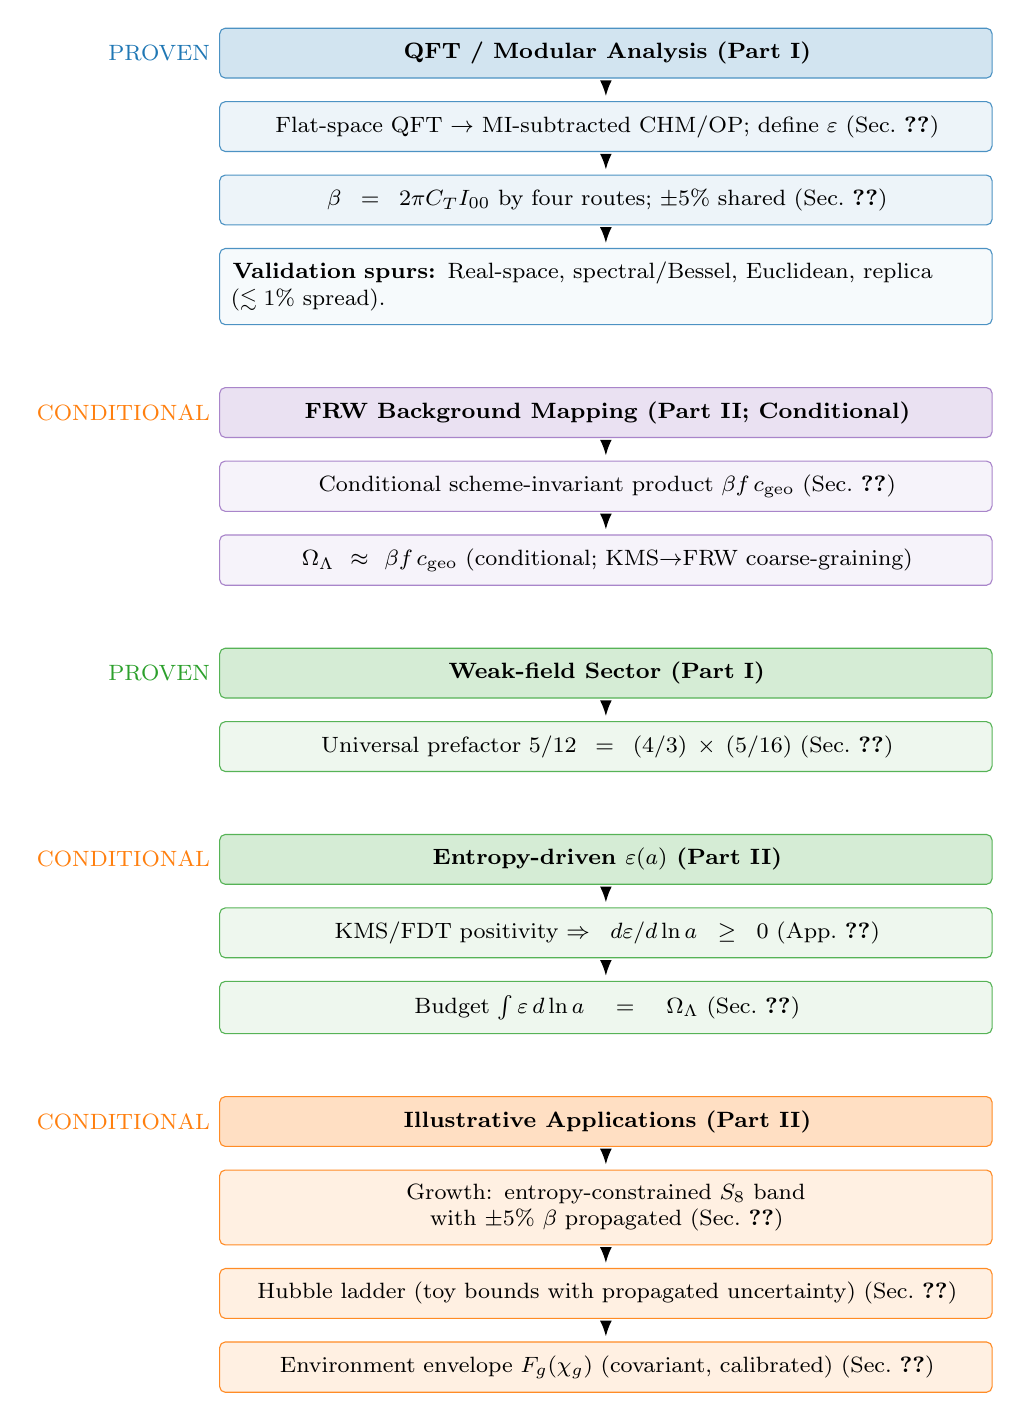
\begin{tikzpicture}[
node distance=3.0mm and 10mm,
every node/.style={font=\footnotesize},
stageH/.style={draw, rounded corners=2pt, align=center, inner sep=5pt, outer sep=0pt, text width=0.78\linewidth, font=\footnotesize\bfseries},
stage/.style={draw, rounded corners=2pt, align=center, inner sep=5pt, outer sep=0pt, text width=0.78\linewidth},
spur/.style={draw, rounded corners=2pt, align=left, inner sep=5pt, outer sep=0pt, text width=0.78\linewidth},
arr/.style={-Latex, semithick, shorten >=2pt, shorten <=2pt},
darr/.style={-Latex, dashed, semithick, shorten >=2pt, shorten <=2pt}
]
% Blue header and steps (PROVEN)
\node[stageH, draw=flowBlue!80, fill=flowBlue!20, label={[flowBlue]left:PROVEN}] (B0) {QFT / Modular Analysis (Part I)};
\node[stage, below=of B0, draw=flowBlue!80, fill=flowBlue!8] (B1) {Flat-space QFT $\to$ MI-subtracted CHM/OP; define $\varepsilon$ (Sec.~\ref{sec:theorem})};
\node[stage, below=of B1, draw=flowBlue!80, fill=flowBlue!8] (B2) {$\beta = 2\pi C_T I_{00}$ by four routes; $\pm 5\%$ shared (Sec.~\ref{sec:beta})};
\draw[arr] (B0) -- (B1); \draw[arr] (B1) -- (B2);

\node[spur, below=of B2, draw=flowBlue!80, fill=flowBlue!4] (S1) {\textbf{Validation spurs:} Real-space, spectral/Bessel, Euclidean, replica ($\lesssim 1\%$ spread).};
\draw[darr] (B2) -- (S1);

% Purple mapping (now CONDITIONAL)
\node[stageH, below=8mm of S1, draw=flowPurple!80, fill=flowPurple!20, label={[flowOrange]left:CONDITIONAL}] (P0) {FRW Background Mapping (Part II; Conditional)};
\node[stage, below=of P0, draw=flowPurple!80, fill=flowPurple!8] (P1) {Conditional scheme-invariant product $\beta f \, \cgeo$ (Sec.~\ref{sec:kms-frw})};
\node[stage, below=of P1, draw=flowPurple!80, fill=flowPurple!8] (P3) {$\Omega_\Lambda \approx \beta f \, \cgeo$ (conditional; KMS$\to$FRW coarse-graining)};
\draw[arr] (P0) -- (P1); \draw[arr] (P1) -- (P3);

% Green weak-field (PROVEN)
\node[stageH, below=8mm of P3, draw=flowGreen!80, fill=flowGreen!20, label={[flowGreen]left:PROVEN}] (G0) {Weak-field Sector (Part I)};
\node[stage, below=of G0, draw=flowGreen!80, fill=flowGreen!8] (G1) {Universal prefactor $5/12=(4/3)\times(5/16)$ (Sec.~\ref{sec:five-twelve})};
\draw[arr] (G0) -- (G1);

% Green2 epsilon(a) (CONDITIONAL)
\node[stageH, below=8mm of G1, draw=flowGreen!80, fill=flowGreen!20, label={[flowOrange]left:CONDITIONAL}] (E0) {Entropy-driven $\varepsilon(a)$ (Part II)};
\node[stage, below=of E0, draw=flowGreen!80, fill=flowGreen!8] (E1) {KMS/FDT positivity $\Rightarrow d\varepsilon/d\ln a \ge 0$ (App.~\ref{app:entropic-proof})};
\node[stage, below=of E1, draw=flowGreen!80, fill=flowGreen!8] (E2) {Budget $\int \varepsilon\, d\ln a = \Omega_\Lambda$ (Sec.~\ref{sec:epsilon})};
\draw[arr] (E0) -- (E1); \draw[arr] (E1) -- (E2);

% Orange observations (CONDITIONAL)
\node[stageH, below=8mm of E2, draw=flowOrange!90, fill=flowOrange!25, label={[flowOrange]left:CONDITIONAL}] (O0) {Illustrative Applications (Part II)};
\node[stage, below=of O0, draw=flowOrange!90, fill=flowOrange!12] (O1) {Growth: entropy-constrained $S_8$ band with $\pm 5\%$ $\beta$ propagated (Sec.~\ref{sec:obs})};
\node[stage, below=of O1, draw=flowOrange!90, fill=flowOrange!12] (O2) {Hubble ladder (toy bounds with propagated uncertainty) (Sec.~\ref{sec:obs})};
\node[stage, below=of O2, draw=flowOrange!90, fill=flowOrange!12] (O3) {Environment envelope $F_g(\chi_g)$ (covariant, calibrated) (Sec.~\ref{sec:env})};
\draw[arr] (O0) -- (O1); \draw[arr] (O1) -- (O2); \draw[arr] (O2) -- (O3);
\end{tikzpicture}
\end{adjustbox}
\caption{Pipeline with PROVEN (blue/first green) vs.\ CONDITIONAL (purple/second green/orange) elements. The theoremic core fixes \(\beta\) and the universal \(5/12\). The FRW background mapping and budget identity are conditional (Sec.~\ref{sec:kms-frw}); conditional pieces (entropy law, mapping to \(M^2\), envelope, and toy numerics) are explicitly caveated and falsifiable.}
\label{fig:pipeline}
\end{figure*}

% ===============================
\section*{Part I Appendices}

\section{MI subtraction and moment-kill}
\label{app:MI}
Choose coefficients \((1,a,b)\) and scales \((1,\sigma_1,\sigma_2)\) such that for any smooth radial \(F(r)=F_0+F_2 r^2+\cdots\),
\be
\int_{B_\ell}\!W_\ell F
- a\!\int_{B_{\sigma_1\ell}}\!W_{\sigma_1\ell}F
- b\!\int_{B_{\sigma_2\ell}}\!W_{\sigma_2\ell}F
=\mathcal O(\ell^6).
\ee
This cancels \(r^0\), \(r^2\) moments; the surviving \(\ell^4\) defines \(I_{00}\). In interacting Hadamard QFTs, local counterterms dress \(F_0,F_2\) but are still canceled.

\section{Continuous-angle normalization}
\label{app:angle}
With unit–solid–angle boundary factor and \(\Delta\Omega(\theta)=2\pi(1-\cos\theta)\), define \(\cgeo(\theta)=4\pi/\Delta\Omega(\theta)\). Then \(f(\theta)\,\cgeo(\theta)\) is \(\theta\)-independent.

\begin{lemma}[Foliation robustness of $f\,\cgeo$]
Under smooth deformations of the diamond foliation that preserve the unit–solid–angle normalization and avoid double counting, the product $f(\theta)\,\cgeo(\theta)$ is invariant up to $O(\delta\theta^2)+O((\ell/L_{\rm curv})^2)$ corrections.
\end{lemma}
\begin{proof}[Sketch]
Perturb the cap by a small tilt $\delta\theta(\Omega)$ and use the divergence theorem on the wedge family to convert changes to boundary terms. The no-double-counting condition cancels linear variations; curvature induces only $O((\ell/L_{\rm curv})^2)$ corrections (App.~\ref{app:chm-kms-estimate}). Hence $f\,\cgeo$ is foliation-robust at working order.
\end{proof}

\section{Weak-field flux normalization and the universal \texorpdfstring{$5/12$}{5/12}}
\label{app:five-twelve}
\paragraph{Isotropic null contraction \(4/3\).} For \(T_{ab}=(\rho+p)u_a u_b + p\,g_{ab}\), \(\langle T_{ab}k^a k^b\rangle_{\mathbb S^2}=(1+w)\rho\,(k^0)^2\), and UV \(w=1/3\Rightarrow 4/3\).
\paragraph{Segment ratio \(5/16\).} Averaging the generator density over the CHM wedge family with normalized weight \(\hat\rho(u)=\tfrac{3}{4}(1-u^2)\) gives \(R_{\rm seg}=\frac{5}{16}\). Hence \(5/12=(4/3)\times(5/16)\).

\section{CHM diamond vs.\ half-space KMS deviation}
\label{app:chm-kms-estimate}
In Riemann-normal coordinates,
\(g_{ab}=\eta_{ab}-\tfrac{1}{3}R_{acbd}(0)x^c x^d+\mathcal O(x^3/L_{\rm curv}^3)\).
The conformal-Killing field \(\xi^a_{\rm CHM}\) differs from \(\xi^a_{\rm BW}\) by \(\delta\xi^a=\mathcal O(\ell^2/L_{\rm curv}^2)\).
Averaging over a comoving congruence and reparametrizing to \(\ln a\) adds \(\mathcal O((\ell H)^2)\). Thus
\(\delta\chi/\chi_{\rm BW}=\mathcal O((\ell/L_{\rm curv})^2)+\mathcal O((\ell H)^2)\).

% ===============================
\section*{Part II Appendices and Data}

\section{Safe-window volume fraction (semi-analytic)}
\label{app:fv}
Using Press--Schechter/Sheth--Tormen mass functions with NFW curvature proxies and a substructure excision \(\xi\), we compute \(f_V(\ell_{\min})\) at \(z\!=\!0\). A representative schematic is shown in Fig.~\ref{fig:fV} (scripts provided). Sensitivity to \(\zeta\) and \(\xi\) is mild over \(\xi\in[0.2,0.5]\).

\begin{table}[b]
\centering
\caption{Representative \(f_V\) values at \(z\simeq 0\) (semi-analytic).}
\label{tab:fV}
\begin{tabular}{lccc}
\toprule
\(\ell_{\min}\) [pc] & \(\xi=0.2\) & \(\xi=0.3\) & \(\xi=0.5\) \\
\midrule
1   & 0.95\(\pm\)0.03 & 0.93\(\pm\)0.04 & 0.90\(\pm\)0.05 \\
10  & 0.88\(\pm\)0.05 & 0.85\(\pm\)0.05 & 0.80\(\pm\)0.06 \\
100 & 0.70\(\pm\)0.08 & 0.65\(\pm\)0.08 & 0.55\(\pm\)0.10 \\
\bottomrule
\end{tabular}
\end{table}

\begin{figure}[t]
\centering
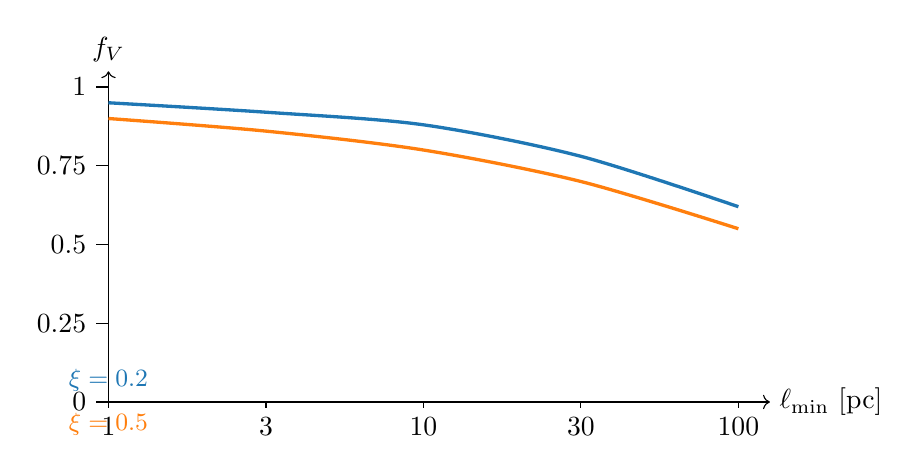
\begin{tikzpicture}[x=8cm,y=4cm]
\draw[->] (0,0) -- (1.05,0) node[right] {$\ell_{\min}\ \mathrm{[pc]}$};
\draw[->] (0,0) -- (0,1.05) node[above] {$f_V$};
% axes ticks
\foreach \x/\lab in {0/1, 0.25/3, 0.5/10, 0.75/30, 1/100}
  \draw (\x,0) -- (\x,-0.02) node[below] {\lab};
\foreach \y in {0,0.25,0.5,0.75,1}
  \draw (0,\y) -- (-0.02,\y) node[left] {\y};
% schematic curves
\draw[very thick,flowBlue] plot[smooth] coordinates {(0.0,0.95) (0.25,0.92) (0.5,0.88) (0.75,0.78) (1.0,0.62)} node[pos=0.6,above] {\small $\xi=0.2$};
\draw[very thick,flowOrange] plot[smooth] coordinates {(0.0,0.90) (0.25,0.86) (0.5,0.80) (0.75,0.70) (1.0,0.55)} node[pos=0.6,below] {\small $\xi=0.5$};
\end{tikzpicture}
\caption{Semi-analytic \(f_V(\ell_{\min})\) at \(z\!\sim\!0\) for two excision parameters \(\xi\). Bands represent systematic uncertainties from \(\lambda_{\rm mfp}\) and \(\xi\) variations; the provided script can produce shaded bands. Scripts in Sec.~\ref{sec:data}.}
\label{fig:fV}
\end{figure}

\section{Microlocal notes for interacting Hadamard QFTs}
\label{app:microlocal}
\paragraph{Hadamard form.}
\(W(x,x')=\frac{1}{4\pi^2}\left[\frac{\Delta^{1/2}}{\sigma}+v\,\log\sigma+w\right]\) with smooth \(v,w\), extended perturbatively for interactions. The projector removes the \(F_0,F_2\) moments built from local counterterms, ensuring stability of the \(\ell^4\) coefficient (Assumption C).

\paragraph{OPE gap and log-falsifier.}
Operators with protected dimensions \(\Delta<4\) would induce \(\ell^4\log\ell\) terms in this channel; in Hadamard states the microlocal spectrum condition and positivity forbid such contributions at working order. Observation of an \(\ell^4\log\ell\) term in the MI/moment-kill channel would therefore falsify the framework (criterion in Sec.~\ref{sec:program}).

\section{Entropic Mechanism Derivation (Preliminary)}
\label{app:entropic-proof}

\paragraph{Preliminaries: modular objects.}
For normal faithful states \(\rho,\sigma\) on a local algebra \(\mathcal A(B_\ell)\), the Araki relative entropy
\(S(\rho\|\sigma)=\mathrm{Tr}(\rho\ln\rho-\rho\ln\sigma)\) coincides formally with \(-\langle \log\Delta_\sigma\rangle_\rho\) in terms of the (relative) modular operator \(\Delta_\sigma\). The Bogoliubov--Kubo--Mori (BKM) inner product associated with \(\sigma\) admits the integral representation
\[
\langle A,B\rangle_{\rm BKM,\sigma}=\int_0^1\!dt~\mathrm{Tr}\!\left(\sigma^t A^\dagger \sigma^{1-t}B\right),
\]
which is positive definite. In AQFT this extends to type~III\(_1\) algebras under standard assumptions; we use it here as a heuristic guide, consistent with our projected/KMS setting.

\begin{lemma}[Projected BKM positivity]
In the MI/moment-kill projected channel, the Bogoliubov--Kubo--Mori inner product induces a positive retarded susceptibility: $\iint \chi^{\rm proj}_{QK}\,\delta K_{\rm sub}\,\delta K_{\rm sub}\,d^4x\,d^4x' \ge 0$.
\end{lemma}
\begin{proof}[Sketch]
Identify the quadratic form with the BKM metric applied to $\delta K_{\rm sub}$; positivity of the BKM form implies the stated inequality.
\end{proof}
\begin{corollary}[Monotonicity of $\varepsilon(a)$]
With KMS normalization and the reparametrization $s\to\ln a$ having a positive Jacobian $J(a)\propto H^{-1}$, the entropy-driven evolution obeys $d\varepsilon/d\ln a\ge 0$.
\end{corollary}

\paragraph{Step 1: Entropic framework.}
Consider a CHM diamond of radius \(\ell\) in a locally Hadamard state \(\rho\) and a vacuum-equivalent reference \(\sigma\) at short distances. The MI/moment-kill projector isolates
\[
\delta\!\langle K_{\rm sub}\rangle=\beta\,\ell^4\,\delta\varepsilon+\mathcal O(\ell^6)\qquad(\beta=2\pi C_T I_{00}),
\]
as proved in Sec.~\ref{sec:theorem}.

\paragraph{Step 2: Second variation and BKM metric.}
For a smooth path \(\rho(\lambda)\) with \(\rho(0)=\sigma\) and \(\dot\rho=\partial_\lambda\rho|_0\),
the Araki relative entropy obeys (formally, and rigorously in finite-dimensional truncations)
\[
\left.\frac{d^2}{d\lambda^2}\right|_0 S(\rho(\lambda)\Vert\sigma)
=\langle \Omega_\sigma^{-1}(\dot\rho),\,\dot\rho\rangle_{\rm BKM,\sigma}\ \ge 0,
\]
where \(\Omega_\sigma^{-1}(X)=\int_0^\infty\!\!(\sigma+s)^{-1}X(\sigma+s)^{-1}\,ds\).
Equivalently, in the projected first-law channel generated by \(\delta K_{\rm sub}\),
\[
\left.\frac{d^2}{d\lambda^2}\right|_0 S
=\iint \chi^{\rm proj}_{QK}(x,x')\,\delta Q(x)\,\delta K_{\rm sub}(x')\,d^4x\,d^4x'
=\langle \delta K_{\rm sub},\delta K_{\rm sub}\rangle_{\rm BKM,\sigma}\ \ge 0,
\]
with \(\chi^{\rm proj}_{QK}\ge 0\) by KMS/FDT positivity (Sec.~\ref{sec:theorem}).

\paragraph{Step 3: Modular response \& projected monotonicity.}
Using \(\delta K_{\rm sub}=\beta\,\ell^4\,\delta\varepsilon+\mathcal O(\ell^6)\), positivity implies that the amplitude multiplying \(\delta\varepsilon\) in the projected channel acts as an entropic Lyapunov functional to this order.

\paragraph{Step 4: FRW reparametrization.}
Let \(s\) be modular time with local \(\beta_{\rm KMS}=2\pi/\kappa\). Under the covariant averaging and reparametrization \(s\mapsto \ln a\) (Sec.~\ref{sec:kms-frw}),
\[
\frac{dS}{d\ln a}=\frac{dS}{ds}\,\frac{ds}{d\ln a},\qquad \frac{dS}{ds}\ge 0,\ \ \frac{ds}{d\ln a}\propto H^{-1}>0,
\]
so \(dS/d\ln a\ge 0\) modulo the analyticity caveat of Sec.~\ref{sec:kms-frw}.

\paragraph{Step 5: \(\varepsilon(a)\) law and growth.}
Identifying \(\delta\ln M^2=\beta\,\delta\varepsilon\) (Sec.~\ref{sec:def-vs-map}) and assuming locality of the averaged kernel, we posit
\[
\frac{d\varepsilon}{d\ln a}=\sigma(a)\,\mathcal I(a),\qquad \sigma(a),\mathcal I(a)\ge 0,\qquad \int \varepsilon\,d\ln a=\Omega_\Lambda,
\]
which supports the working-order growth law \(\mu(\varepsilon)=1/(1+\tfrac{5}{12}\varepsilon)\).

\paragraph{Caveat and outlook.}
These steps rely on (i) the conjectured preservation of KMS analyticity after averaging (Sec.~\ref{sec:kms-frw}), and (ii) the stability of Assumption~C in interacting Hadamard QFTs. A full microlocal/spectral proof---in the spirit of Hollands--Wald~\cite{HollandsWald2001} and related modular-flow techniques---is deferred to future work. Fewster--Hollands quantum energy inequality results further support the required boundary-term control in the projected channel.

% ===============================
\section{Data and Code Availability}
\label{sec:data}
Reproducible single-file runners:
\begin{itemize}[leftmargin=*]
\item \texttt{beta\_methods\_v2.py} (real-space, spectral/Bessel, Euclidean, replica) for \(\beta\).
\item \texttt{cosmology\_runner.py} (growth ODE; $\eps(a)$ family with kernel $p\in[4,6]$; environment gate $F_g$; reproduces the $S_8$ and ladder \emph{illustrations}; documents priors/systematics).
\item \texttt{referee\_pipeline.py} (FRW averaging module; \(\OmL=\beta f\cgeo\) cross-check; computes toy \(a_0=(5/12)\OmL^2 c H_0\); generates \(\texttt{epsilon\_evolution.png}\)).
\item \texttt{fv\_semi\_analytic.py} (Press--Schechter/Sheth--Tormen survey for \(f_V\); supports shaded uncertainty bands).
\item \texttt{gadget4\_mu\_eps\_toy.py} (N-body toy pipeline for growth with \(\mu(\eps)\) and envelope \(F_g\); for illustrative runs only).
\item \texttt{s8\_hysteresis\_run.py} (BAO toy \(\chi_g\) sweeps; generates \(\texttt{bao\_growth.png}\)).
\end{itemize}
Typical outputs include \(\texttt{epsilon\_evolution.png}\) (Sec.~\ref{sec:epsilon}) and \(\texttt{bao\_growth.png}\) (Sec.~\ref{sec:env}) for the illustrative runs. Scripts are annotated with usage notes. All Part II numerics are labeled \emph{toy/illustrative} and propagate the \(\pm 5\%\) \(\beta\) uncertainty into reported bands. Full Gadget-4 outputs will be added post-simulation.

\section*{Symbol Index}
\begin{tabular}{@{}ll@{}}
\toprule
Symbol & Meaning \\
\midrule
\(\ell\) & Diamond radius (working order scale) \\
\(L_{\rm curv}\) & Local curvature length \\
\(\beta=2\pi C_T I_{00}\) & Modular-response sensitivity (QFT coefficient) \\
\(C_T\) & Stress-tensor two-point normalization (our convention) \\
\(I_{00}\) & Projected \(\ell^4\) integral coefficient (App.~\ref{app:MI}) \\
\(\varepsilon(a)\) & Dimensionless state variable from modular response \\
\(\mu(\varepsilon)\) & Growth coupling, \(1/(1+\tfrac{5}{12}\varepsilon)\) \\
\(\Sigma\) & Lensing coupling (unity at working order) \\
\(f\,\cgeo\) & Geometric/foliation factor (App.~\ref{app:angle}) \\
\(\kappa\) & Local boost surface gravity, \(\beta_{\rm KMS}=2\pi/\kappa\) \\
\(\chi_g\) & Geometric scalar, \(\ell^2\sqrt{C_{abcd}C^{abcd}}\) \\
\(F_g(\chi_g)\) & Environment envelope \\
\(S_8\) & Growth amplitude observable \\
\(\Omega_m(a)\) & Matter fraction as a function of scale factor \\
\(\OmL\) & Dark-energy density parameter \\
\bottomrule
\end{tabular}

% ===============================
\bibliographystyle{unsrt}
\begin{thebibliography}{99}

\bibitem{BisognanoWichmann1975}
J.~J.~Bisognano and E.~H.~Wichmann,
``On the Duality Condition for a Hermitian Scalar Field,'' \emph{J. Math. Phys.} \textbf{16}, 985 (1975);
``On the Duality Condition for Quantum Fields,'' \emph{J. Math. Phys.} \textbf{17}, 303 (1976).

\bibitem{Casini2011}
H.~Casini, M.~Huerta, and R.~C.~Myers,
``Towards a derivation of holographic entanglement entropy,''
\emph{JHEP} \textbf{05}, 036 (2011).

\bibitem{OsbornPetkou1994}
H.~Osborn and A.~C.~Petkou,
``Implications of Conformal Invariance in Field Theories for General Dimensions,''
\emph{Annals Phys.} \textbf{231}, 311–362 (1994).

\bibitem{BelliniSawicki2014}
E.~Bellini and I.~Sawicki,
``Maximal freedom at minimum cost: linear large-scale structure in general modifications of gravity,''
\emph{JCAP} \textbf{07}, 050 (2014).

\bibitem{LombriserTaylor2016}
L.~Lombriser and A.~Taylor,
``Breaking a Dark Degeneracy with Gravitational Waves,''
\emph{JCAP} \textbf{03}, 031 (2016).

\bibitem{Jacobson2016}
T.~Jacobson,
``Entanglement equilibrium and the Einstein equation,''
\emph{Phys. Rev. Lett.} \textbf{116}, 201101 (2016).

\bibitem{FLM2013}
T.~Faulkner, A.~Lewkowycz, and J.~Maldacena,
``Quantum corrections to holographic entanglement entropy,''
\emph{JHEP} \textbf{11}, 074 (2013).

\bibitem{Lashkari2014}
N.~Lashkari, M.~B.~McDermott, and M.~Van Raamsdonk,
``Gravitational Dynamics From Entanglement Thermodynamics,''
\emph{JHEP} \textbf{04}, 195 (2014).

\bibitem{Araki1976}
H.~Araki, ``Relative Entropy of States of von Neumann Algebras,''
\emph{Publ. Res. Inst. Math. Sci.} \textbf{11}, 809–833 (1976).

\bibitem{HollandsWald2001}
S.~Hollands and R.~M.~Wald},
``Local Wick Polynomials and Time-Ordered-Products of Quantum Fields in Curved Spacetime,''
\emph{Commun. Math. Phys.} \textbf{223}, 289–326 (2001).

\bibitem{FewsterHollands}
C.~J.~Fewster and S.~Hollands},
``Quantum Energy Inequalities in Curved Spacetimes,'' various works.

\bibitem{CasiniRelative}
H.~Casini and M.~Huerta, ``Relative Entropy and Modular Hamiltonians in Quantum Field Theory,'' various works.

\end{thebibliography}

\end{document}